\section{Seguimiento}

\subsection{Introducción}

La salida del bloque de reconstrucción, son los puntos 3D generados a partir de los múltiples vídeos de cada vista, presentados en el orden que fueron validados en cada frame (figura \ref{reconstr_00}).

Son presentados arbitrariamente para cada cuadro de la secuencia, y el objetivo del tracking o seguimiento, es identificarlos temporalmente, asignándoles una etiqueta constante para obtener las trayectorias 3D de cada marcador.

\begin{figure}[hbt]
\begin{center}
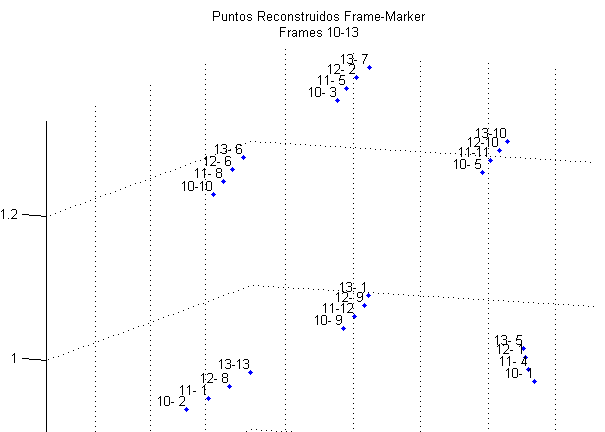
\includegraphics[scale=0.8]{img/Tracking/00_Salida_Reconstruccion}
\end{center}
\caption{Salida de Reconstrucción para 4 frames. La etiqueta para cada marcador es el indice en la reconstrucción para un determinado frame}
\label{reconstr_00}
% Figura tomada de la reconstruccion 8_07_100_200
\end{figure}

El procedimiento presentado \cite{herda} , es aplicar el tracking de partículas esbozado por Malik,Dracos,Papantoniou \cite{griegos} al seguimiento de marcadores. El mismo consiste en buscar el desplazamiento de un marcador desde el cuadro [f] al cuadro siguiente [f+1], sobre una ventana de cuatro cuadros. 

La hipótesis principal de este procedimiento, es que el muestreo del movimiento capturado  es suficiente para que el desplazamiento entre cuadros sea mínimo en distancia, y la idea para predecir y buscar el desplazamiento entre [f] y [f+1], es utilizar la información que se tiene de la secuencia entre [f-1] y [f], y utilizar una segunda proyección entre [f+1] y [f+2] para confirmar el enlace encontrado en el caso que exista mas de una posibilidad (figura \ref{herda_00}). El muestreo se considera constante, por lo cual podemos realizar las derivadas discretas de las trayectorias.

Para poder confirmar una trayectoria de 4 puntos, se debe cumplir que la misma presenta la menor variación de aceleración para la opción elegida entre todas las posibles, calculada como:

\begin{equation}
\begin{split}
\Delta{a}&= \left| \boldsymbol{\overrightarrow{a}}_{[f][f+1][f+2]}-\boldsymbol{\overrightarrow{a}}_{[f-1][f][f+1]} \right| \\
&= \left| \left(\boldsymbol{\overrightarrow{v}}_{[f+1][f+2]}-\boldsymbol{\overrightarrow{v}}_{[f][f+1]}\right).\Delta{t}-\left(\boldsymbol{\overrightarrow{v}}_{[f][f+1]}-\boldsymbol{\overrightarrow{v}}_{[f-1][f]}\right).\Delta{t} \right| \\
&= \left|\left( x_{[f+2]} - 3.x_{[f+1]} + 3.x_{[f]} - x_{[f-1]} \right).\Delta{t}^2\right|\\
\end{split}
\label{track_var_acc}
\end{equation}

, donde $x_{[f+1]}$ a su vez, es aquel punto de [f+1] que mejor se aproxima al desplazamiento en frames anteriores, minimizando la ecuación \ref{track_acc} 

\begin{equation}
\begin{split}
\boldsymbol{\overrightarrow{v}}_{[f][f+1]}& = \boldsymbol{\overrightarrow{v}}_{[f-1][f]} \\
x_{[f+1]}-x_{[f]}& = x_{[f]}-x_{[f-1]} \\
\end{split}
\label{track_acc}
\end{equation}

\begin{figure}[hbt]
\begin{center}
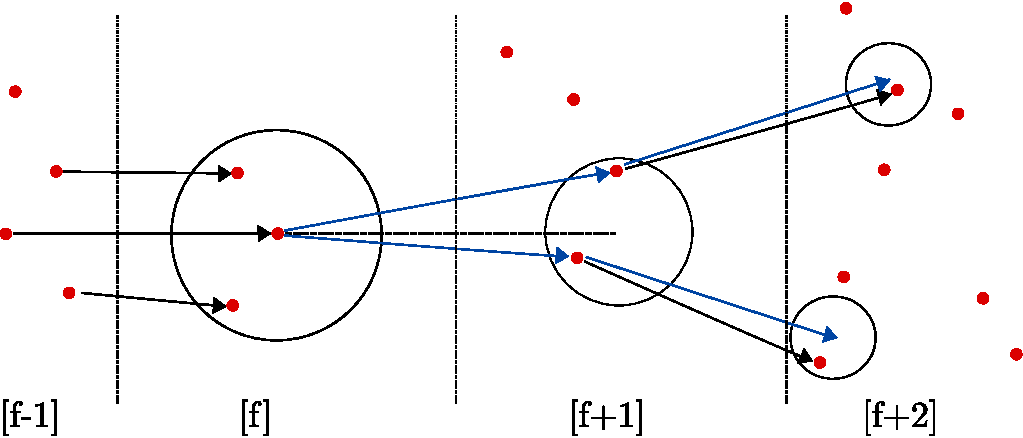
\includegraphics[scale=0.8]{img/Tracking/tracking-eps-converted-to.pdf}
\end{center}
\caption{Seguimiento en 4 frames, siendo [f] el frame actual que queremos seguir en [f+1]. La linea punteada es la traslación del movimiento previo, las lineas azules son las obtenidas buscando la mínima variación de aceleración para el punto elegido en [f+1]. De las dos posibles trayectorias, se elige aquella con menor variación de aceleración}
\label{herda_00}
\end{figure}

En su trabajo\cite{herda}, Lorna Herda propone que realizar el seguimiento sobre la reconstrucción 3D presenta menos continuidad en las trayectorias , con respecto al seguimiento realizado sobre el conjunto de segmentación sumada a la proyección de los puntos reconstruidos 3D en cada vista 2D. Sin embargo, en nuestras pruebas, nos pareció mas coherente trabajar con el seguimiento en los puntos reconstruidos en 3D, ya que en caso de trayectorias que se cruzan en una vista 2D, son fácilmente separadas en 3D debido a la geometría. 

Adicionalmente, la reconstrucción fue implementada de forma distinta a la propuesta por Herda, si bien es posible obtener los puntos proyectados en cada vista, no cumplen el mismo rol. 

(Comparación Imagen de Tracking 2D, sobre 3D)

Finalmente, asumiendo que los puntos obtenidos directamente de las animaciones ,proyectados en cada cámara, son el mejor caso de puntos 2D, no presentaban grandes ventajas de trabajar el enlace en cada una de estas vistas 2D, sobre trabajar en 3D posteriormente a la reconstrucción, y no volver hacia atrás ya que la geometría entre vistas cumplió su cometido. Esto ultimo no se cumple para el caso que se evalúen medidas adicionales para robustecer la salida del tracking (ejemplo: validacion por visibilidad), como se estudiará en las conclusiones.

\subsection{Implementación}

Para un frame [f] y un marcador $m_{i}^{[f]}$, se desea encontrar en el frame [f+1] el marcador $m_{j}^{[f+1]}$ que continúe la trayectoria que se tiene hasta el momento, cumpliendo las ecuaciones de continuidad \ref{track_acc} y \ref{track_var_acc}. El elemento que traslada la informacion de un frame al siguiente y desde el anterior, es la matriz de enlaces, donde cada linea es un enlace, y cada enlace tiene los siguientes elementos:
\begin{equation}
\begin{bmatrix}
  m_{h}^{[f-1]} ,\quad m_{i}^{[f]} ,\quad m_{j}^{[f+1]} ,\quad m_{k}^{[f+2]} ,\quad \left|\boldsymbol{\overrightarrow{a}}_{[f-1][f][f+1]}\right| ,\quad \left|\boldsymbol{\overrightarrow{v}}_{[f][f+1]}\right|
\end{bmatrix}
\end{equation}

Para el ejemplo presentado en la figura \ref{reconstr_00} , en frame $f=11$ el marcador $m=8$ presenta el siguiente enlace hacia $(f+1)=12$, 

\begin{equation}
\begin{bmatrix}
  m_{3}^{[10]} ,\quad m_{8}^{[11]} ,\quad m_{3}^{[12]} ,\quad N/A ,\quad \left|\boldsymbol{\overrightarrow{a}}_{[10][11][12]}\right| ,\quad \left|\boldsymbol{\overrightarrow{v}}_{[1][12]}\right|
\end{bmatrix}
\end{equation}

, donde el indice en [13] no aplica debido a que no fue necesario para establecer en enlace entre [11][12].

Al final de cada iteración, la matriz de enlaces es consolidada para asignarle a cada nuevo marcador en [f+1] la etiqueta definida en el primer cuadro del enlazado, la cual puede ser inicializada como texto, si se le presenta la opción al usuario (en caso contrario, se utiliza el orden de los marcadores en el primer frame). Esta asignación será la que se utilice a lo largo de todo el seguimiento, por lo que todo marcador que no sea reconstruido en los primero frames, salvo de tomen medidas adicionales, no aparecerán en las trayectorias finales.

\subsubsection{Enlazado en régimen}

Dado un frame [f], se cargan todos los marcadores de los frames [f-1],[f],[f+1],[f+2], los cuales son puntos en coordenadas cartesianas $X,Y,Z$ (si el seguimiento desea hacerse para una vista 2D, se establece la tercer coordenada de todos los puntos en 1) en unidades correspondiente al plano donde se trabaja (pixeles para vistas 2D, metros para espacio 3D). Dentro de cada frame, los marcadores son identificados según su indice en la reconstrucción, y los enlaces de cada marcador [f-1][f], son cargados a partir de la matriz de enlace del frame anterior (la segunda y tercer columna de la matriz de enlace de [f-1], presenta los mismos datos que la primer y segunda columna de la matriz de enlace en [f], salvo el orden en que es presentada que es asociado al frame en curso).

Para el $i$-esimo marcador en [f], se relevan los indices que componen el enlace [f-1][f] para obtener el traslado previo, y aplicarlo para obtener el centro de búsqueda para el marcador en [f], cumpliendo la ecuación \ref{track_acc} .

\begin{equation}
\begin{split}
\boldsymbol{\overrightarrow{v}}_{[f][f+1]}^{i} = \boldsymbol{\overrightarrow{v}}_{[f-1][f]}^{i} \Rightarrow C_{[f+1]}^{i} &= x_{[f]}^{i} + \boldsymbol{\overrightarrow{v}}_{[f-1][f]}^{i}.\Delta{t} \\
&= 2.x_{[f]}^{i} -x_{[f-1]}^{i} 
\end{split}
\label{centro_busqueda_f1}
\end{equation}

La norma de este traslado es utilizada para evaluar los puntos cercanos al centro de búsqueda, donde pueden surgir tres casos:

\begin{itemize}
\item Se encuentra un solo punto dentro del radio de búsqueda , se agrega el indice del punto encontrado en [f+1] a los que se utilizaron de [f-1] y [f], calculando la aceleración y velocidad resultante para establecer el enlace. En este caso, el cuarto elemento de la linea de la matriz de enlace, no fue necesario 
\item Se encuentra mas de un punto, por lo cual se tiene que usar algún criterio para elegir entre todas la posibilidades encontradas. Para cada punto encontrado dentro del radio de búsqueda, se calcula un segundo centro de búsqueda para [f+2], esta vez minimizando la ecuación \ref{track_var_acc} :
\begin{equation}
\begin{split}
\boldsymbol{\overrightarrow{a}}_{[f][f+1][f+2]}=\boldsymbol{\overrightarrow{a}}_{[f-1][f][f+1]} \Rightarrow C_{[f+2]}^{i} &= x_{[f+1]}^{i} + \boldsymbol{\overrightarrow{v}}_{[f][f+1]}^{i}.\Delta{t} + \boldsymbol{\overrightarrow{a}}_{[f-1][f][f+1]}^{i}.\Delta{t}^2\\
&= 3.x_{[f+1]}^{i} - 3.x_{[f]}^{i} + x_{[f-1]}^{i}\end{split}
\label{centro_busqueda_f2}
\end{equation}
, siendo el radio de búsqueda en [f+2], la distancia [f][f+1]. Con los puntos encontrados en cada búsqueda de todas las posibilidades, se evalúa la variación de aceleración para los puntos [f-1][f][f+1][f+2], y elige la menor de todas, estableciendo el enlace de 4 puntos. Finalmente, se calcula la aceleración y velocidad del enlace [f-1][f][f+2], y se guardan los indices que permitieron la decisión, esta vez con cuatro elementos para indicar que se procedió con la segunda búsqueda.
\item No se encuentra ningún punto, tanto para la búsqueda en [f+1] como en [f+2]. En este caso, se presentan múltiples alternativas, en distintas etapas. La mas inmediata durante el enlazado frame a frame, es aumentar el radio de búsqueda (por ejemplo puede suceder con un punto acelerando y fuera del radio de búsqueda). Este aumento puede ser limitado, o indefinido hasta encontrar un punto aunque en una distancia mucho mayor a la esperada, por lo que deben ser validados posteriormente. Si el enlace pasa la validación dentro del frame, puede no pasar una validación posterior de trayectoria lo que se verá mas adelante
\end{itemize}




\subsubsection{Enlazado inicial y final}



\subsubsection{Validación e Inventario de trayectorias}

Antes de consolidar la matriz de enlaces y proceder a que los marcadores en [f+1] hereden las etiquetas de las trayectorias a las que pertenecen, los enlaces deben ser validados en múltiples instancias:

\begin{itemize}
\item \textbf{Validación dentro del frame}: verificar que los indices de la matriz de enlaces en [f+1] son únicos, asociados a una sola trayectoria. Si dos o mas trayectorias se enlazaron a un mismo punto en [f+1], se comparará la aceleración con la que fueron enlazadas, validando aquella con menor aceleración, y descartando las otras. En este punto , existe la posibilidad de haber agregado todas las trayectorias involucradas en la decisión en vez de una sola trayectoria por marcador en [f+1], que mejor cumplía las condiciones para ese marcador. De haber elegido esta opción, el descartar una trayectoria que podría haber sido elegida por menor variación , daría paso a la siguiente mejor. Este caso sucedía mas en los casos que se aplico el seguimiento para trayectorias 2D, no tanto en 3D, por lo cual se terminó procediendo con solo una trayectoria por marcador, la cual en caso de ser invalida debe ser evaluada en la etapa de inventario de trayectorias  
\item \textbf{Validación en trayectoria}: pueden existir puntos que fueron reconstruidos con leves errores que deben detectarse, corregirse y estimar un reemplazo. Estos puntos son detectados como enlazados correctamente, pero con posición, velocidad, o aceleración que presenta una discontinuidad notoria, como puede observarse en el ejemplo de la figura \ref{discontinuidad_tracking} ,

\begin{figure}[H]
 \centering
  \subfloat[Trayectoria]{
   \label{track_m13}
    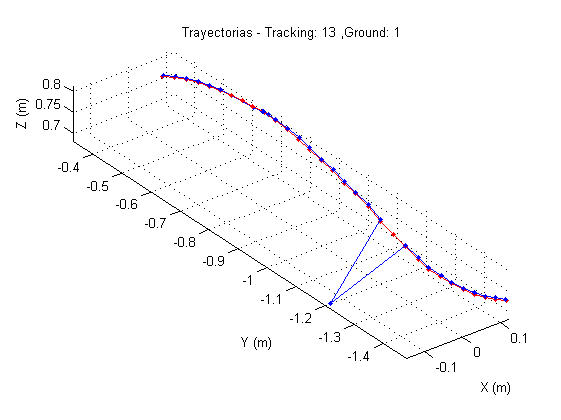
\includegraphics[width=0.5\textwidth]{img/Tracking/025_Salida_Tracking_Marker_13_8_07_100_200.png}}
  \subfloat[Velocidad,Aceleración,Variación Ac.]{
   \label{vel_acc_vacc_m13}
    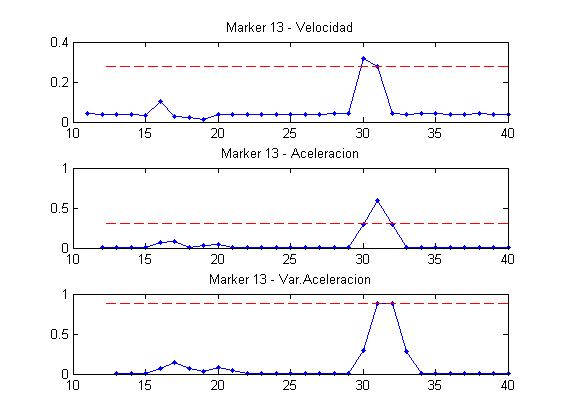
\includegraphics[width=0.5\textwidth]{img/Tracking/020_Salida_Tracking_Marker_13_8_07_100_200.png}}
 \caption{Ejemplo de discontinuidad en un marcador, por punto mal reconstruido. La figura \ref{track_m13} presenta en azul la trayectoria reconstruida, en rojo el ground truth}
 \label{discontinuidad_tracking}
\end{figure}

Se establece un umbral a partir del estudio de la distribucion de la aceleracion de cada marcador (figura \ref{distribucion_aceleracion} ) para encontrar la aceleracion que presenta un salto abrupto, y detectar los frames donde se supera dicho umbral para corregir el marcador. El procedimiento para estimar los marcadores en estos casos, es el mismo que se verá al momento de inventario de trayectorias.
\begin{figure}[H]
 \centering
  \subfloat[Funcion de distribucion de la Aceleracion]{
	\label{distribucion_aceleracion}
	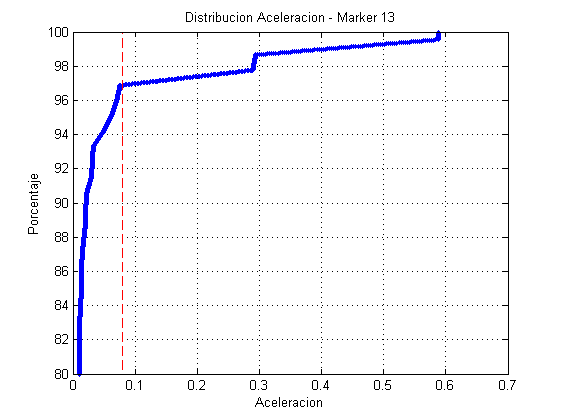
\includegraphics[width=0.5\textwidth]{img/Tracking/03_Distribucion_Aceleracion_Marker_13_8_07_100_200.png}}
  \subfloat[]{
   \label{track_m13_fix}
    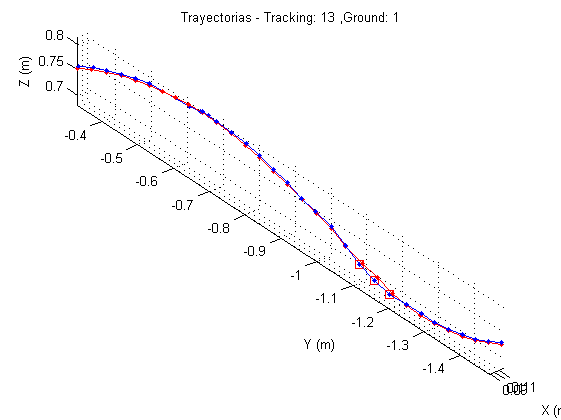
\includegraphics[width=0.5\textwidth]{img/Tracking/026_Salida_Tracking_Marker_13_8_07_100_200.png}}
 \caption{Ejemplo Resultado de Umbral y Correcion En Trayectoria}
% Figura tomada de la reconstruccion 8_07_100_200
\label{distro_acc_track_m13_fix}
\end{figure}
\item \textbf{Inventario de Trayectorias}: Durante el enlazado en un frame, se tienen marcadores en [f] que no lograron enlazarse en [f+1], pero cuya trayectoria podría estar enlazada hasta este frame.
Estos puntos deben ser identificados, mediante la comparacion de la segunda columna de la matriz de enlaces [f][f+1] (actual) y la tercer columna de la matriz de enlaces [f-1][f] (anterior), ya que ambas tienen informacion de los marcadores en el mismo frame, pero enlazan hacia atras y adelante.
Los elementos que se encuentren en la matriz [f-1][f] , pero no hayan sido enlazados en [f][f+1], son agregados a una lista que  contiene hasta que momneto el frame mantenía el enlace (ultima vez que se tuvo informacion de la trayectoria a la cual pertenece), y que indice de marcador tenia en ese momento (pasar de indice en un frame, a trayectoria a la cual pertenece es trivial consultando las etiquetas de marcador que se van heredando de frame a frame).

Una vez actualizada la lista de las trayectorias perdidas en [f][f+1], se deben tratar de enlazar los puntos de [f+1] que no entraron en el enlazado regular, con las trayectorias perdidas hasta [f-1]. Todos los puntos que sobraron en el enlazado regular, son evaluados contra la lista de trayectorias perdidas, y se revisan dos condiciones:

\begin{enumerate}
  \item Distancia con respecto a una estimación lineal, prolongando el movimiento tomando el ultimo punto como inicio, y los ultimos frames de la trayectoria conocida como desplazamiento. El despalzamiento es repetido tantas veces como tiempo perdido tiene el marcador: si una trayectoria estaba definida hasta [f-1] y se buscan enlaces con elementos de [f+1], el desplazamiento es repetido dos veces, como puede observarse en el ejemplo de la figure \ref{track_m8_recover}. 
 
\begin{figure}[H]
 \centering
  \subfloat[Salida de Codigo durante perdida y recuperación de trayectoria]{
	\label{track_m8_recover_code}
	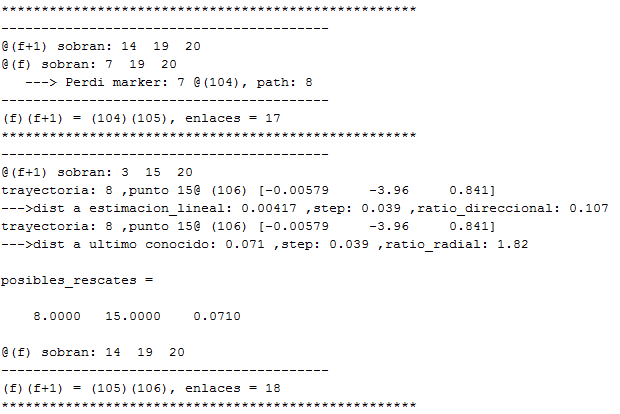
\includegraphics[scale=0.7]{img/Tracking/035_Salida_Codigo_Recuperacion.png}}\hspace{3 mm}
	
  \subfloat[Trayectoria]{
   \label{track_m8_recover}
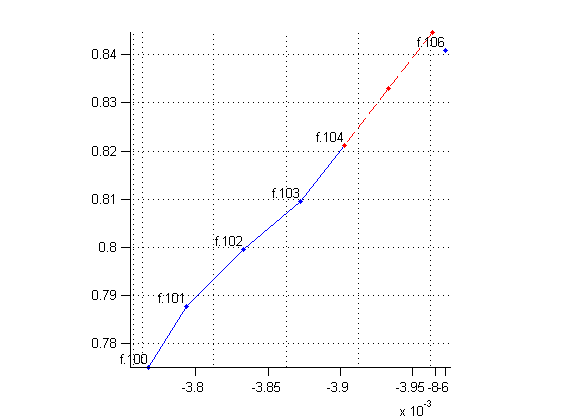
\includegraphics[scale=0.7]{img/Tracking/030_Inventario_trayectoria_direccional.png}}
\caption{Trayectoria perdida en frame 104, con posible candidato de recuperacion en frame 106 por cercania con la estimacion por desplazamiento}
% Figura tomada de la reconstruccion 8_07_100_200
\label{inventario_trayectoria_direccional}
\end{figure} 
  
  \item Distancia radial con respecto al ultimo punto conocido. En algunos casos, la perdida del enlazado puede suceder cuando la trayectoria está en reposo (por ejemplo, un pie apoyado antes de volver a despegarse del suelo), o en transicion (en el medio de una curva), por lo cual la estimacion lineal anterior es invalida. Para ello, es útil relevar la distancia entre el ultimo punto conocido de una trayectoria trunca, y los puntos que no se enlazaron en [f+1]. Esta distancia, en caso de una posible recuperacion, debera ser proporcional al ultimo traslado conocido, por la diferencia temporal de frames entre el ultimo punto, y el posible candidato.
  
\end{enumerate} 

\end{itemize}

Si se encuentra algún punto que cumpla alguna de estas condiciones, es considerado para continuar la trayectoria, y deben estimarse los puntos intermedios para completar la trayectoria.

Esta estimación es realizada mediante minimos cuadrados, donde las condiciones iniciales dependen de cuantos puntos de la trayectoria se tenían hasta el momento, la condicion final es el punto encontrado en [f+1], las incognitas son los puntos intermedios que se quieren encontrar, y las multiples ecuaciones a cumplir son las planteadas en (\ref{track_var_acc}) y (\ref{track_acc}).

Sea $X_{[f+1]}$ un punto candidato por las condiciones anteriores, y el ultimo punto conocido en [f-1] de un trayectoria que pretende continuar, verifica [f-1]$\geq$3, entonces las ecuaciones que el punto a estimar $\boldsymbol{\tilde{X}_{[f]}}$ deberá cumplir, (observar que las ecuaciones de variacion de aceleracion son combinacion lineal de las ecuaciones de aceleracion)

\begin{equation}
\left\{
\begin{matrix}
X_{[f-3]} &-3.X_{[f-2]} &+3.X_{[f-1]} &-\boldsymbol{\tilde{X}_{[f]}} & &=0 \\
 &X_{[f-2]} &-3.X_{[f-1]} &+3.\boldsymbol{\boldsymbol{\tilde{X}_{[f]}}} &-X_{[f+1]} &=0 \\
 &X_{[f-2]} &-2.X_{[f-1]} &+\boldsymbol{\boldsymbol{\tilde{X}_{[f]}}} & &=0 \\
 & &X_{[f-1]} &-2.\boldsymbol{\boldsymbol{\tilde{X}_{[f]}}} &+X_{[f+1]} &=0 \\
\end{matrix}
\right.
\label{ecuaciones_estimacion_01}
\end{equation}

, escribiendo de forma matricial, separando los datos en incognitas y condiciones,

\begin{equation}
\begin{split}
&\begin{pmatrix}
1 &-3 &3 &-1&0\\
0 &1 &-3 &3 &-1\\
0 &1 &-2 &1 &0\\
0 &0 &1 &-2 &1\\
\end{pmatrix}
\begin{pmatrix}
X_{[f-3]}\\
X_{[f-2]}\\
X_{[f-1]}\\
\boldsymbol{\tilde{X}_{[f]}}\\
X_{[f+1]}\\
\end{pmatrix} =
\begin{pmatrix}
1 &-3 &3\\
0 &1 &-3\\
0 &1 &-2\\
0 &0 &1\\
\end{pmatrix}
\begin{pmatrix}
X_{[f-3]}\\
X_{[f-2]}\\
X_{[f-1]}\\
\end{pmatrix}+
\begin{pmatrix}
-1\\
3\\
1\\
-2\\
\end{pmatrix}
\boldsymbol{\tilde{X}_{[f]}}+
\begin{pmatrix}
0\\
-1\\
0\\
1\\
\end{pmatrix}
X_{[f+1]} = 
\begin{pmatrix}
0\\
0\\
0\\
0\\
\end{pmatrix} \\
&\Rightarrow
\underbrace{
\begin{pmatrix}
-1\\
3\\
1\\
-2\\
\end{pmatrix}
}_{A_{[f]}}\boldsymbol{\tilde{X}_{[f]}} = \underbrace{- \begin{pmatrix}
1 &-3 &3\\
0 &1 &-3\\
0 &1 &-2\\
0 &0 &1\\
\end{pmatrix}
\begin{pmatrix}
X_{[f-3]}\\
X_{[f-2]}\\
X_{[f-1]}\\
\end{pmatrix} - \begin{pmatrix}
0\\
-1\\
0\\
1\\
\end{pmatrix}
X_{[f+1]}}_{B_{[f]}} \\
&\Rightarrow \boldsymbol{\tilde{X}_{[f]}} = \left( A_{[f]}^{t}.A_{[f]}\right)^{-1}.A_{[f]}^{t}.B_{[f]}
\end{split}
\label{matrices_estimacion_01}
\end{equation}




\subsection{Resultado y Analisis}


